
%(BEGIN_QUESTION)
% Copyright 2012, Tony R. Kuphaldt, released under the Creative Commons Attribution License (v 1.0)
% This means you may do almost anything with this work of mine, so long as you give me proper credit

The following FOUNDATION Fieldbus function block program implements a ``cascade'' stragety where a temperature controller sends a setpoint to a flow controller, which in turn positions a control valve:

$$\includegraphics[width=15.5cm]{i02135x01.eps}$$

Identify where each scheduled communication event (i.e. CD token) must take place in order to execute this Fieldbus program, identifying which signal paths in the function block diagram are communicated this way.  Note: you may simply put a check-mark or some other indicating symbol next to the signal lines you identify in the diagram.

\underbar{file i02135}
%(END_QUESTION)





%(BEGIN_ANSWER)

{\it 3 points for the line between FT-213 and the slave PID block, 3 points for the line between the master PID's output and the slave PID's cascade input, and 4 points for the BKCAL line from the slave PID block to the master PID block.}

$$\includegraphics[width=15.5cm]{i02135x02.eps}$$

%(END_ANSWER)





%(BEGIN_NOTES)

{\bf This question is intended for exams only and not worksheets!}.

%(END_NOTES)


